\resizebox{0.98\textwidth}{!}{%
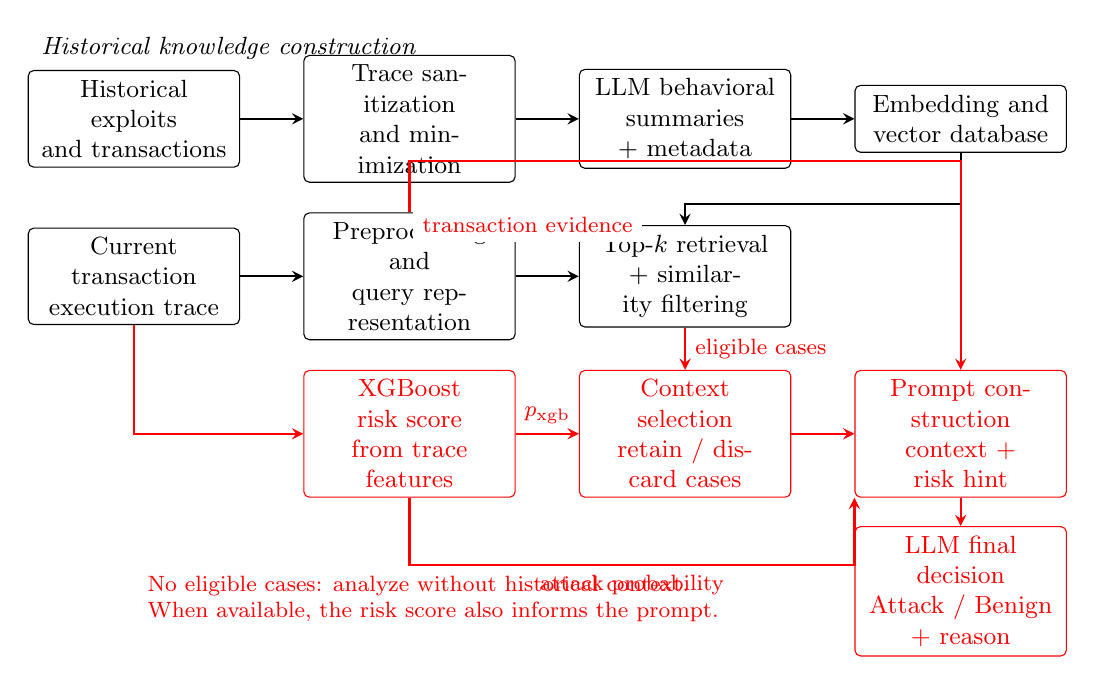
\begin{tikzpicture}[x=1cm,y=1cm,>=stealth,font=\small,
box/.style={draw,rounded corners=2pt,align=center,minimum height=.85cm,text width=2.45cm},
changed/.style={box,draw=red,text=red},arr/.style={->,thick}]
\node[box] (exploit) at (0,0) {Historical exploits\\and transactions};
\node[box] (trace) at (3.5,0) {Trace sanitization\\and minimization};
\node[box] (summary) at (7,0) {LLM behavioral\\summaries + metadata};
\node[box] (kb) at (10.5,0) {Embedding and\\vector database};
\draw[arr] (exploit)--(trace); \draw[arr] (trace)--(summary); \draw[arr] (summary)--(kb);
\node[anchor=west,font=\small\itshape] at (-1.3,.9) {Historical knowledge construction};
\node[box] (input) at (0,-2) {Current transaction\\execution trace};
\node[box] (prune) at (3.5,-2) {Preprocessing and\\query representation};
\node[box] (retrieve) at (7,-2) {Top-$k$ retrieval\\+ similarity filtering};
\draw[arr] (input)--(prune); \draw[arr] (prune)--(retrieve);
\draw[arr] (kb.south)--++(0,-.65)-|(retrieve.north);
\node[changed] (xgb) at (3.5,-4) {XGBoost risk score\\from trace features};
\node[changed] (gate) at (7,-4) {Context selection\\retain / discard cases};
\node[changed] (prompt) at (10.5,-4) {Prompt construction\\context + risk hint};
\node[changed] (llm) at (10.5,-6) {LLM final decision\\Attack / Benign + reason};
\draw[arr,red] (input.south)|-(xgb.west);
\draw[arr,red] (retrieve.south)--node[right,text=red,font=\footnotesize]{eligible cases}(gate.north);
\draw[arr,red] (xgb)--node[above,font=\footnotesize]{$p_{\mathrm{xgb}}$}(gate);
\draw[arr,red] (gate)--(prompt);
\draw[arr,red] (xgb.south)--++(0,-.85)-|node[pos=.25,below,font=\footnotesize]{attack probability}(prompt.south west);
\draw[arr,red] (prune.north)--++(0,.65)-|(prompt.north);
\node[text=red,font=\footnotesize,fill=white] at (5,-1.35) {transaction evidence};
\draw[arr,red] (prompt)--(llm);
\node[align=left,text=red,font=\footnotesize] at (3.8,-6.1) {No eligible cases: analyze without historical context.\\When available, the risk score also informs the prompt.};
\end{tikzpicture}}
